\documentclass{article}
\usepackage{lmodern}
\usepackage[T1]{fontenc}
\usepackage{shapepar}
\usepackage{microtype}
\usepackage{lipsum}
\usepackage{pgfplots}
\pgfplotsset{compat=1.9}
\usepackage{tikz}
\usetikzlibrary{calc,fit,intersections,folding}
\usepackage{pstricks-add}
\usetikzlibrary{arrows.meta,angles,arrows,quotes,backgrounds}
\usepackage[a3paper,left=5mm,right=5mm,top=25mm,bottom=25mm]{geometry} % Ränder

\newcommand{\tubecolor}{blue}
\newcommand{\thickness}{0.5mm}
\newcommand{\n}{2.5mm}

\begin{document}
\thispagestyle{empty}
\begin{center}
    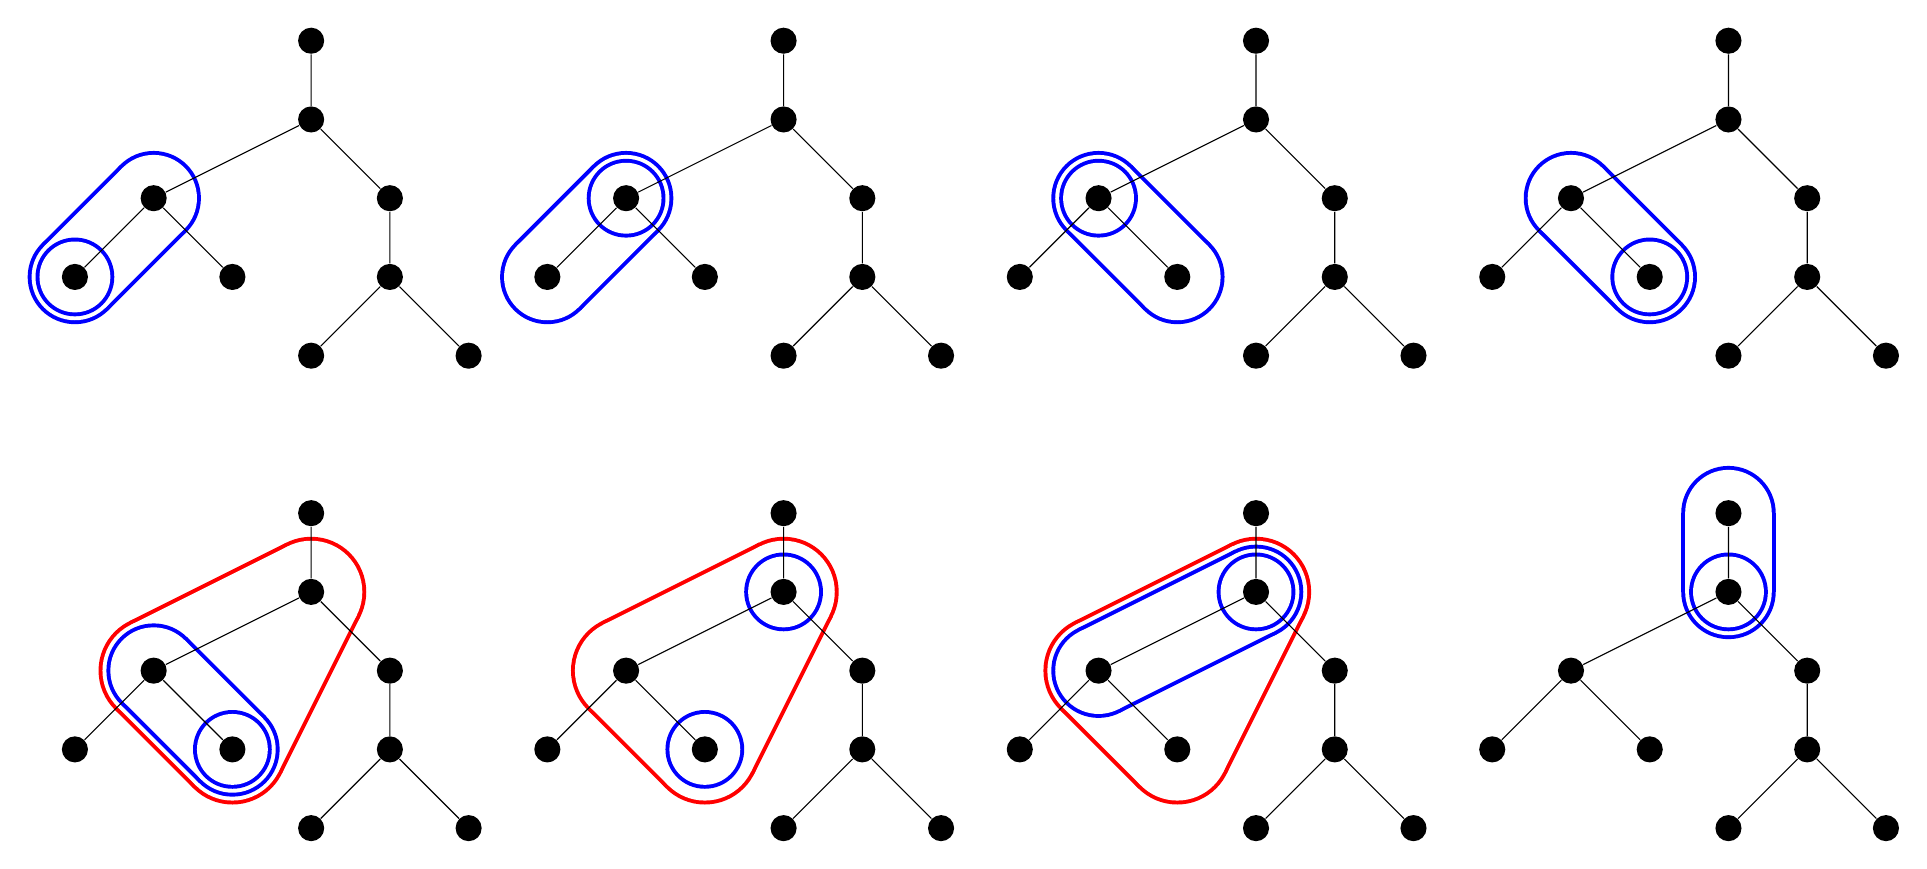
\begin{tikzpicture}
    \begin{scope}
        \node[fill] (1) at (0,0) [circle] {};
        \node[fill] (2) at (0,-1) [circle] {};
        \node[fill] (3) at (1,-2) [circle] {};
        \node[fill] (4) at (1,-3) [circle] {};
        \node[fill] (5) at (0,-4) [circle] {};
        \node[fill] (6) at (-2,-2) [circle] {};
        \node[fill] (7) at (-3,-3) [circle] {};
        \node[fill] (8) at (-1,-3) [circle] {};
        \node[fill] (9) at (2,-4) [circle] {};
        \draw (2) -- (6) -- (7) (6) -- (8) (4) -- (9);
        \draw (1) -- (2) -- (3) -- (4) -- (5);

        %Tube 67
        \begin{scope}[on background layer]
            \fill[\tubecolor] (6) circle (\n + 7*\thickness);
            \fill[\tubecolor] (7) circle (\n + 7*\thickness);
            \draw[\tubecolor] [line width = 2*(\n + 7*\thickness)] (6.center) -- (7.center);
            
            \fill[white] (6) circle (\n + 6*\thickness);
            \fill[white] (7) circle (\n + 6*\thickness);
            \draw[white] [line width = 2*(\n + 6*\thickness)] (6.center) -- (7.center);
        \end{scope}

        %Tube 7
        \begin{scope}[on background layer]
            \fill[\tubecolor] (7) circle (\n + 5*\thickness);
            
            \fill[white] (7) circle (\n + 4*\thickness);
        \end{scope}
    \end{scope}
    
    \begin{scope}[xshift = 6cm]
        \node[fill] (1) at (0,0) [circle] {};
        \node[fill] (2) at (0,-1) [circle] {};
        \node[fill] (3) at (1,-2) [circle] {};
        \node[fill] (4) at (1,-3) [circle] {};
        \node[fill] (5) at (0,-4) [circle] {};
        \node[fill] (6) at (-2,-2) [circle] {};
        \node[fill] (7) at (-3,-3) [circle] {};
        \node[fill] (8) at (-1,-3) [circle] {};
        \node[fill] (9) at (2,-4) [circle] {};
        \draw (2) -- (6) -- (7) (6) -- (8) (4) -- (9);
        \draw (1) -- (2) -- (3) -- (4) -- (5);

        %Tube 67
        \begin{scope}[on background layer]
            \fill[\tubecolor] (6) circle (\n + 7*\thickness);
            \fill[\tubecolor] (7) circle (\n + 7*\thickness);
            \draw[\tubecolor] [line width = 2*(\n + 7*\thickness)] (6.center) -- (7.center);
            
            \fill[white] (6) circle (\n + 6*\thickness);
            \fill[white] (7) circle (\n + 6*\thickness);
            \draw[white] [line width = 2*(\n + 6*\thickness)] (6.center) -- (7.center);
        \end{scope}

        %Tube 6
        \begin{scope}[on background layer]
            \fill[\tubecolor] (6) circle (\n + 5*\thickness);
            
            \fill[white] (6) circle (\n + 4*\thickness);
        \end{scope}
    \end{scope}

    \begin{scope}[xshift = 12cm]
        \node[fill] (1) at (0,0) [circle] {};
        \node[fill] (2) at (0,-1) [circle] {};
        \node[fill] (3) at (1,-2) [circle] {};
        \node[fill] (4) at (1,-3) [circle] {};
        \node[fill] (5) at (0,-4) [circle] {};
        \node[fill] (6) at (-2,-2) [circle] {};
        \node[fill] (7) at (-3,-3) [circle] {};
        \node[fill] (8) at (-1,-3) [circle] {};
        \node[fill] (9) at (2,-4) [circle] {};
        \draw (2) -- (6) -- (7) (6) -- (8) (4) -- (9);
        \draw (1) -- (2) -- (3) -- (4) -- (5);

        %Tube 68
        \begin{scope}[on background layer]
            \fill[\tubecolor] (6) circle (\n + 7*\thickness);
            \fill[\tubecolor] (8) circle (\n + 7*\thickness);
            \draw[\tubecolor] [line width = 2*(\n + 7*\thickness)] (6.center) -- (8.center);
            
            \fill[white] (6) circle (\n + 6*\thickness);
            \fill[white] (8) circle (\n + 6*\thickness);
            \draw[white] [line width = 2*(\n + 6*\thickness)] (6.center) -- (8.center);
        \end{scope}

        %Tube 6
        \begin{scope}[on background layer]
            \fill[\tubecolor] (6) circle (\n + 5*\thickness);
            
            \fill[white] (6) circle (\n + 4*\thickness);
        \end{scope}
    \end{scope}


    \begin{scope}[xshift = 18cm]
        \node[fill] (1) at (0,0) [circle] {};
        \node[fill] (2) at (0,-1) [circle] {};
        \node[fill] (3) at (1,-2) [circle] {};
        \node[fill] (4) at (1,-3) [circle] {};
        \node[fill] (5) at (0,-4) [circle] {};
        \node[fill] (6) at (-2,-2) [circle] {};
        \node[fill] (7) at (-3,-3) [circle] {};
        \node[fill] (8) at (-1,-3) [circle] {};
        \node[fill] (9) at (2,-4) [circle] {};
        \draw (2) -- (6) -- (7) (6) -- (8) (4) -- (9);
        \draw (1) -- (2) -- (3) -- (4) -- (5);

        %Tube 68
        \begin{scope}[on background layer]
            \fill[\tubecolor] (6) circle (\n + 7*\thickness);
            \fill[\tubecolor] (8) circle (\n + 7*\thickness);
            \draw[\tubecolor] [line width = 2*(\n + 7*\thickness)] (6.center) -- (8.center);
            
            \fill[white] (6) circle (\n + 6*\thickness);
            \fill[white] (8) circle (\n + 6*\thickness);
            \draw[white] [line width = 2*(\n + 6*\thickness)] (6.center) -- (8.center);
        \end{scope}

        %Tube 8
        \begin{scope}[on background layer]
            \fill[\tubecolor] (8) circle (\n + 5*\thickness);
            
            \fill[white] (8) circle (\n + 4*\thickness);
        \end{scope}
    \end{scope}

    \begin{scope}[xshift = 0cm, yshift = -6cm]
        \node[fill] (1) at (0,0) [circle] {};
        \node[fill] (2) at (0,-1) [circle] {};
        \node[fill] (3) at (1,-2) [circle] {};
        \node[fill] (4) at (1,-3) [circle] {};
        \node[fill] (5) at (0,-4) [circle] {};
        \node[fill] (6) at (-2,-2) [circle] {};
        \node[fill] (7) at (-3,-3) [circle] {};
        \node[fill] (8) at (-1,-3) [circle] {};
        \node[fill] (9) at (2,-4) [circle] {};
        \draw (2) -- (6) -- (7) (6) -- (8) (4) -- (9);
        \draw (1) -- (2) -- (3) -- (4) -- (5);

        %Tube 268
        \begin{scope}[on background layer]
            \fill[red] (6) circle (\n + 9*\thickness);
            \fill[red] (8) circle (\n + 9*\thickness);
            \fill[red] (2) circle (\n + 9*\thickness);
            \draw[red] [line width = 2*(\n + 9*\thickness)] (6.center) -- (8.center) (8.center) -- (2.center) (2.center) -- (6.center);
            
            \fill[white] (6) circle (\n + 8*\thickness);
            \fill[white] (8) circle (\n + 8*\thickness);
            \fill[white] (2) circle (\n + 8*\thickness);
            \draw[white] [line width = 2*(\n + 8*\thickness)] (6.center) -- (8.center) (8.center) -- (2.center) (2.center) -- (6.center);
            \fill[white] (2.center) -- (6.center) -- (8.center);
        \end{scope}

        %Tube 68
        \begin{scope}[on background layer]
            \fill[\tubecolor] (6) circle (\n + 7*\thickness);
            \fill[\tubecolor] (8) circle (\n + 7*\thickness);
            \draw[\tubecolor] [line width = 2*(\n + 7*\thickness)] (6.center) -- (8.center);
            
            \fill[white] (6) circle (\n + 6*\thickness);
            \fill[white] (8) circle (\n + 6*\thickness);
            \draw[white] [line width = 2*(\n + 6*\thickness)] (6.center) -- (8.center);
        \end{scope}

        %Tube 8
        \begin{scope}[on background layer]
            \fill[\tubecolor] (8) circle (\n + 5*\thickness);
            
            \fill[white] (8) circle (\n + 4*\thickness);
        \end{scope}
    \end{scope}

    \begin{scope}[xshift = 6cm, yshift = -6cm]
        \node[fill] (1) at (0,0) [circle] {};
        \node[fill] (2) at (0,-1) [circle] {};
        \node[fill] (3) at (1,-2) [circle] {};
        \node[fill] (4) at (1,-3) [circle] {};
        \node[fill] (5) at (0,-4) [circle] {};
        \node[fill] (6) at (-2,-2) [circle] {};
        \node[fill] (7) at (-3,-3) [circle] {};
        \node[fill] (8) at (-1,-3) [circle] {};
        \node[fill] (9) at (2,-4) [circle] {};
        \draw (2) -- (6) -- (7) (6) -- (8) (4) -- (9);
        \draw (1) -- (2) -- (3) -- (4) -- (5);

        %Tube 268
        \begin{scope}[on background layer]
            \fill[red] (6) circle (\n + 9*\thickness);
            \fill[red] (8) circle (\n + 9*\thickness);
            \fill[red] (2) circle (\n + 9*\thickness);
            \draw[red] [line width = 2*(\n + 9*\thickness)] (6.center) -- (8.center) (8.center) -- (2.center) (2.center) -- (6.center);
            
            \fill[white] (6) circle (\n + 8*\thickness);
            \fill[white] (8) circle (\n + 8*\thickness);
            \fill[white] (2) circle (\n + 8*\thickness);
            \draw[white] [line width = 2*(\n + 8*\thickness)] (6.center) -- (8.center) (8.center) -- (2.center) (2.center) -- (6.center);
            \fill[white] (2.center) -- (6.center) -- (8.center);
        \end{scope}

        
        %Tube 2
        \begin{scope}[on background layer]
            \fill[\tubecolor] (2) circle (\n + 5*\thickness);
            
            \fill[white] (2) circle (\n + 4*\thickness);
        \end{scope}

        %Tube 8
        \begin{scope}[on background layer]
            \fill[\tubecolor] (8) circle (\n + 5*\thickness);
            
            \fill[white] (8) circle (\n + 4*\thickness);
        \end{scope}
    \end{scope}

    \begin{scope}[xshift = 12cm, yshift = -6cm]
        \node[fill] (1) at (0,0) [circle] {};
        \node[fill] (2) at (0,-1) [circle] {};
        \node[fill] (3) at (1,-2) [circle] {};
        \node[fill] (4) at (1,-3) [circle] {};
        \node[fill] (5) at (0,-4) [circle] {};
        \node[fill] (6) at (-2,-2) [circle] {};
        \node[fill] (7) at (-3,-3) [circle] {};
        \node[fill] (8) at (-1,-3) [circle] {};
        \node[fill] (9) at (2,-4) [circle] {};
        \draw (2) -- (6) -- (7) (6) -- (8) (4) -- (9);
        \draw (1) -- (2) -- (3) -- (4) -- (5);

        %Tube 268
        \begin{scope}[on background layer]
            \fill[red] (6) circle (\n + 9*\thickness);
            \fill[red] (8) circle (\n + 9*\thickness);
            \fill[red] (2) circle (\n + 9*\thickness);
            \draw[red] [line width = 2*(\n + 9*\thickness)] (6.center) -- (8.center) (8.center) -- (2.center) (2.center) -- (6.center);
            
            \fill[white] (6) circle (\n + 8*\thickness);
            \fill[white] (8) circle (\n + 8*\thickness);
            \fill[white] (2) circle (\n + 8*\thickness);
            \draw[white] [line width = 2*(\n + 8*\thickness)] (6.center) -- (8.center) (8.center) -- (2.center) (2.center) -- (6.center);
            \fill[white] (2.center) -- (6.center) -- (8.center);
        \end{scope}

        %Tube 26
        \begin{scope}[on background layer]
            \fill[\tubecolor] (6) circle (\n + 7*\thickness);
            \fill[\tubecolor] (2) circle (\n + 7*\thickness);
            \draw[\tubecolor] [line width = 2*(\n + 7*\thickness)] (6.center) -- (2.center);
            
            \fill[white] (6) circle (\n + 6*\thickness);
            \fill[white] (2) circle (\n + 6*\thickness);
            \draw[white] [line width = 2*(\n + 6*\thickness)] (6.center) -- (2.center);
        \end{scope}

        %Tube 2
        \begin{scope}[on background layer]
            \fill[\tubecolor] (2) circle (\n + 5*\thickness);
            
            \fill[white] (2) circle (\n + 4*\thickness);
        \end{scope}
    \end{scope}

    \begin{scope}[xshift = 18cm, yshift = -6cm]
        \node[fill] (1) at (0,0) [circle] {};
        \node[fill] (2) at (0,-1) [circle] {};
        \node[fill] (3) at (1,-2) [circle] {};
        \node[fill] (4) at (1,-3) [circle] {};
        \node[fill] (5) at (0,-4) [circle] {};
        \node[fill] (6) at (-2,-2) [circle] {};
        \node[fill] (7) at (-3,-3) [circle] {};
        \node[fill] (8) at (-1,-3) [circle] {};
        \node[fill] (9) at (2,-4) [circle] {};
        \draw (2) -- (6) -- (7) (6) -- (8) (4) -- (9);
        \draw (1) -- (2) -- (3) -- (4) -- (5);

        %Tube 12
        \begin{scope}[on background layer]
            \fill[\tubecolor] (1) circle (\n + 7*\thickness);
            \fill[\tubecolor] (2) circle (\n + 7*\thickness);
            \draw[\tubecolor] [line width = 2*(\n + 7*\thickness)] (1.center) -- (2.center);
            
            \fill[white] (1) circle (\n + 6*\thickness);
            \fill[white] (2) circle (\n + 6*\thickness);
            \draw[white] [line width = 2*(\n + 6*\thickness)] (1.center) -- (2.center);
        \end{scope}

        %Tube 2
        \begin{scope}[on background layer]
            \fill[\tubecolor] (2) circle (\n + 5*\thickness);
            
            \fill[white] (2) circle (\n + 4*\thickness);
        \end{scope}
    \end{scope}

\end{tikzpicture}
\end{center}
\end{document}